\documentclass{article}

\usepackage{fancyhdr}
\usepackage{extramarks}
\usepackage{amsmath}
\usepackage{amsthm}
\usepackage{amsfonts}

% TikZ/Graphics
\usepackage{tikz}
\usetikzlibrary{
    automata,  % for markov chains
    arrows.meta,  % arrow tips (technically deprecated)
    backgrounds,  % background layers
    decorations,  % decorations applied to paths
    decorations.markings,  % additional markings on paths
    decorations.pathmorphing,  % deforming decorations
    decorations.pathreplacing,  % replacing paths
    calligraphy,  % for calligraphic brace (must be loaded after decorations)
    patterns,  % patterns for filling areas
    positioning,  % better custom positioning
    shapes,  % various shapes
    intersections,
}
\usepackage{forest}
\usepackage{circuitikz}
\usepackage{pgfplots}
\pgfplotsset{compat=1.18}
\usepgfplotslibrary{
    groupplots,  % grouping pgf plots
}

\usepackage[plain]{algorithm}
\usepackage{algpseudocode}
\usepackage{hyperref}
\usepackage{multicol}
\usepackage{mathrsfs}
\usepackage{pifont}
\usepackage{circledsteps}

\usetikzlibrary{automata,positioning}

%
% Basic Document Settings
%

\topmargin=-0.45in
\evensidemargin=0in
\oddsidemargin=0in
\textwidth=6.5in
\textheight=9.0in
\headsep=0.25in

\linespread{1.1}

\pagestyle{fancy}
\lhead{\hmwkAuthorName}
\chead{\hmwkClass\ (\hmwkClassInstructor): \hmwkTitle}
\rhead{\firstxmark}
\lfoot{\lastxmark}
\cfoot{\thepage}

\renewcommand\headrulewidth{0.4pt}
\renewcommand\footrulewidth{0.4pt}

\setlength\parindent{0pt}

%
% Create Problem Sections
%

\newcommand{\enterProblemHeader}[1]{
    \nobreak\extramarks{}{Problem \arabic{#1} continued on next page\ldots}\nobreak{}
    \nobreak\extramarks{Problem \arabic{#1} }{Problem \arabic{#1} continued on next page\ldots}\nobreak{}
}

\newcommand{\exitProblemHeader}[1]{
    \nobreak\extramarks{Problem \arabic{#1} }{Problem \arabic{#1} continued on next page\ldots}\nobreak{}
    \stepcounter{#1}
    \nobreak\extramarks{Problem \arabic{#1}}{}\nobreak{}
}

\setcounter{secnumdepth}{0}
\newcounter{partCounter}
\newcounter{homeworkProblemCounter}
\setcounter{homeworkProblemCounter}{1}
\nobreak\extramarks{Problem \arabic{homeworkProblemCounter}}{}\nobreak{}

%
% Homework Problem Environment
%
% This environment takes an optional argument. When given, it will adjust the
% problem counter. This is useful for when the problems given for your
% assignment aren't sequential. See the last 3 problems of this template for an
% example.
%
\newenvironment{homeworkProblem}[2][-1]{
    \ifnum#1>0
        \setcounter{homeworkProblemCounter}{#1}
    \fi
    \section{Problem \arabic{homeworkProblemCounter}: #2}
    \setcounter{partCounter}{1}
    \enterProblemHeader{homeworkProblemCounter}
}{
    \exitProblemHeader{homeworkProblemCounter}
}

%
% Homework Details
%   - Title
%   - Due date
%   - Class
%   - Section/Time
%   - Instructor
%   - Author
%

\newcommand{\hmwkTitle}{Homework\ \#3}
\newcommand{\hmwkDueDate}{February 15, 2025}
\newcommand{\hmwkClass}{Discrete Mathematics}
\newcommand{\hmwkClassTime}{Section A}
\newcommand{\hmwkClassInstructor}{Professor Satish Rao}
\newcommand{\hmwkAuthorName}{\textbf{Zachary Brandt}}
\newcommand{\hmwkAuthorEmail}{\href{mailto:zbrandt@berkeley.edu}{zbrandt@berkeley.edu}}

%
% Title Page
%

\title{
    \vspace{2in}
    \textmd{\textbf{\hmwkClass:\ \hmwkTitle}}\\
    \normalsize\vspace{0.1in}\small{Due\ on\ \hmwkDueDate\ at 4:00pm}\\
    \vspace{0.1in}\large{\textit{\hmwkClassInstructor}}
    \vspace{3in}
}

\author{\hmwkAuthorName \\ \hmwkAuthorEmail}
\date{}

\renewcommand{\part}[1]{\textbf{\large Part \Alph{partCounter}}\stepcounter{partCounter}\\}

%
% Various Helper Commands
%

% Useful for algorithms
\newcommand{\alg}[1]{\textsc{\bfseries \footnotesize #1}}

% For derivatives
\newcommand{\deriv}[1]{\frac{\mathrm{d}}{\mathrm{d}x} (#1)}

% For partial derivatives
\newcommand{\pderiv}[2]{\frac{\partial}{\partial #1} (#2)}

% Integral dx
\newcommand{\dx}{\mathrm{d}x}

% Alias for the Solution section header
\newcommand{\solution}{\textbf{\large Solution}}

% Probability commands: Expectation, Variance, Covariance, Bias
\newcommand{\E}{\mathrm{E}}
\newcommand{\Var}{\mathrm{Var}}
\newcommand{\Cov}{\mathrm{Cov}}
\newcommand{\Bias}{\mathrm{Bias}}

\begin{document}

\maketitle

\pagebreak

% \begin{homeworkProblem}{Edge Colorings}

    An edge coloring of a graph is an assignment of colors to edges in a graph 
    where any two edges incident to the same vertex have different colors. An 
    example is shown on the left.

    \begin{center}
        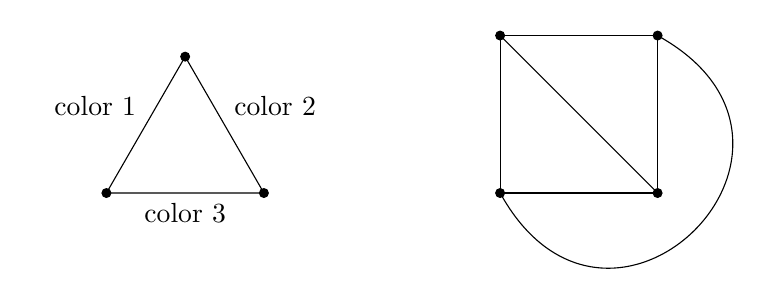
\begin{tikzpicture}
            \clip (-1, -1) rectangle (8, 2.1);
    
            \node[circ] (n1) at (0, 0) {};
            \node[circ] (n2) at (1, {sqrt(3)}) {};
            \node[circ] (n3) at (2, 0) {};
            \draw (n1) -- node[above left] {color 1} (n2)
            -- node[above right] {color 2} (n3)
            -- node[below] {color 3} (n1);
    
            \node[circ] (m1) at (5, 0) {};
            \node[circ] (m2) at (5, 2) {};
            \node[circ] (m3) at (7, 2) {};
            \node[circ] (m4) at (7, 0) {};
            \draw (m1) -- (m2) -- (m3) -- (m4) -- (m1);
            \draw (m2) -- (m4);
            \draw (m1) edge[out=-60, in=-30, looseness=2.5] (m3);
        \end{tikzpicture}
    \end{center}

    \begin{itemize}
        \item[A)] Show that the 4 vertex complete graph above can be 3 edge colored.
        (You may use the numbers $1,2,3$ for colors. A figure is shown on the right.)
        \item[B)] Prove that any graph with maximum degree $d \geq 1$ can be edge 
        colored with $2d-1$ colors. 
        \item[C)] Prove that a tree can be edge colored with $d$ colors where $d$
         is the maximum degree of any vertex.
    \end{itemize}

    \part 

    Below is the 4-vertex graph with edges colored such that only 3 colors are used.

    \begin{flushleft}
        \begin{tikzpicture}
            \clip (-1, -1) rectangle (8, 2.1);
    
            \node[circ] (m1) at (5, 0) {};
            \node[circ] (m2) at (5, 2) {};
            \node[circ] (m3) at (7, 2) {};
            \node[circ] (m4) at (7, 0) {};
            \draw[red, thick] (m1) -- (m2);
            \draw[blue, thick] (m2) -- (m3);
            \draw[red, thick] (m3) -- (m4);
            \draw[blue, thick] (m4) -- (m1);
            \draw[brown, thick] (m2) -- (m4);
            \draw[brown, thick] (m1) edge[out=-60, in=-30, looseness=2.5] (m3);
        \end{tikzpicture}
    \end{flushleft}

    \part 
    % Since a graph can be edge colored when any two edges incident to the same 
    % vertex have different colors, any graph with maximum degree $d \geq 1$ can
    % be edge colored with $2d-1$ colors. $2d-1$ is always greater than or equal 
    % to $d$ when $d \geq 1$, and it is always possible to 

    To prove that any graph with maximum degree $d \geq 1$ can be edge colored with
    $2d -1$ colors I will use the principle of induction on $d$. 

    \begin{itemize}
        \item \textit{Base case}: When the maximum degree of a graph is $d=1$ 
        there can only be two vertices and one edge. It therefore only takes $2d
        - 1 = 2(1)-1 = 1$ colors to color the edges and the claim holds. 
        \item \textit{Inductive hypothesis}: Assume that any graph with maximum 
        degree $d \geq 1$ can be edge colored with $2d-1$ colors for some $1 \leq d 
        \leq k$ where $k \in \mathbb{N}$
        \item \textit{Inductive step}: For $d = k + 1$, we can show that any graph
        can be edge colored with $2d -1$ colors. There exists at least one vertex
        with degree $k+1$, which we can remove along with its incident edges. The
        remaining graph has a maximum degree of $k$, since the other vertices lost 
        their connection and dropped in degree. By the inductive hypothesis, the 
        remaining graph can be edge colored with $2k-1$ colors. Coloring the graph
        with the removed vertex requires $k+1$ colors (one color for each edge).
        There are $2(k+1)-1=2k+1$ colors at our disposal, which is enough to color
        each edge uniquely. Therefore, the graph can be colored with $2(k+1)-1$
        colors. Therefore, any graph with maximum degree $d \geq 1$ can be edge
        colored with $2d-1$ colors.
    \end{itemize}

    \part 

    I prove that a tree can be edge colored with $d$ colors where $d$ is the
    maximum degree of any vertex using the principle of induction on the number
    of vertices in the tree, $n$. 

    \begin{itemize}
        \item \textit{Base case}: When there are two vertices, there is only one
        edge to color, and so can be colored in $d$ colors, since the maximum 
        degree of either vertex is 1.
        \item \textit{Inductive hypothesis}: Assume that the claim holds for any
        tree with vertices $2 \leq n \leq k$.
        \item \textit{Inductive step}: Remove any one of the leaves of the tree, 
        i.e. a vertex of degree 1 alongisde its edge. By the inductive hypothesis, 
        this tree can be colored with $d$ colors. For the parent of this leaf vertex,
        its maximum degree is $d-1$ after removing the edge, and there is at least one
        color for all the edges such that it can be edge colored, with one extra one 
        as $d - (d-1) = 1$. Therefore, there is a color remaining for the leaf and edge
        that was removed to be colored. Therefore the claim has been proven true for all 
        trees with $n$ vertices. 
    \end{itemize}

    
\end{homeworkProblem}
\begin{homeworkProblem}{Edge Colorings}

    An edge coloring of a graph is an assignment of colors to edges in a graph 
    where any two edges incident to the same vertex have different colors. An 
    example is shown on the left.

    \begin{center}
        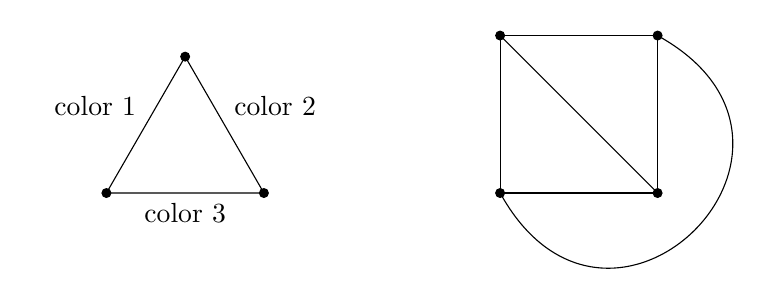
\begin{tikzpicture}
            \clip (-1, -1) rectangle (8, 2.1);
    
            \node[circ] (n1) at (0, 0) {};
            \node[circ] (n2) at (1, {sqrt(3)}) {};
            \node[circ] (n3) at (2, 0) {};
            \draw (n1) -- node[above left] {color 1} (n2)
            -- node[above right] {color 2} (n3)
            -- node[below] {color 3} (n1);
    
            \node[circ] (m1) at (5, 0) {};
            \node[circ] (m2) at (5, 2) {};
            \node[circ] (m3) at (7, 2) {};
            \node[circ] (m4) at (7, 0) {};
            \draw (m1) -- (m2) -- (m3) -- (m4) -- (m1);
            \draw (m2) -- (m4);
            \draw (m1) edge[out=-60, in=-30, looseness=2.5] (m3);
        \end{tikzpicture}
    \end{center}

    \begin{itemize}
        \item[A)] Show that the 4 vertex complete graph above can be 3 edge colored.
        (You may use the numbers $1,2,3$ for colors. A figure is shown on the right.)
        \item[B)] Prove that any graph with maximum degree $d \geq 1$ can be edge 
        colored with $2d-1$ colors. 
        \item[C)] Prove that a tree can be edge colored with $d$ colors where $d$
         is the maximum degree of any vertex.
    \end{itemize}

    \part 

    Below is the 4-vertex graph with edges colored such that only 3 colors are used.

    \begin{flushleft}
        \begin{tikzpicture}
            \clip (-1, -1) rectangle (8, 2.1);
    
            \node[circ] (m1) at (5, 0) {};
            \node[circ] (m2) at (5, 2) {};
            \node[circ] (m3) at (7, 2) {};
            \node[circ] (m4) at (7, 0) {};
            \draw[red, thick] (m1) -- (m2);
            \draw[blue, thick] (m2) -- (m3);
            \draw[red, thick] (m3) -- (m4);
            \draw[blue, thick] (m4) -- (m1);
            \draw[brown, thick] (m2) -- (m4);
            \draw[brown, thick] (m1) edge[out=-60, in=-30, looseness=2.5] (m3);
        \end{tikzpicture}
    \end{flushleft}

    \part 
    % Since a graph can be edge colored when any two edges incident to the same 
    % vertex have different colors, any graph with maximum degree $d \geq 1$ can
    % be edge colored with $2d-1$ colors. $2d-1$ is always greater than or equal 
    % to $d$ when $d \geq 1$, and it is always possible to 

    To prove that any graph with maximum degree $d \geq 1$ can be edge colored with
    $2d -1$ colors I will use the principle of induction on $d$. 

    \begin{itemize}
        \item \textit{Base case}: When the maximum degree of a graph is $d=1$ 
        there can only be two vertices and one edge. It therefore only takes $2d
        - 1 = 2(1)-1 = 1$ colors to color the edges and the claim holds. 
        \item \textit{Inductive hypothesis}: Assume that any graph with maximum 
        degree $d \geq 1$ can be edge colored with $2d-1$ colors for some $1 \leq d 
        \leq k$ where $k \in \mathbb{N}$
        \item \textit{Inductive step}: For $d = k + 1$, we can show that any graph
        can be edge colored with $2d -1$ colors. There exists at least one vertex
        with degree $k+1$, which we can remove along with its incident edges. The
        remaining graph has a maximum degree of $k$, since the other vertices lost 
        their connection and dropped in degree. By the inductive hypothesis, the 
        remaining graph can be edge colored with $2k-1$ colors. Coloring the graph
        with the removed vertex requires $k+1$ colors (one color for each edge).
        There are $2(k+1)-1=2k+1$ colors at our disposal, which is enough to color
        each edge uniquely. Therefore, the graph can be colored with $2(k+1)-1$
        colors. Therefore, any graph with maximum degree $d \geq 1$ can be edge
        colored with $2d-1$ colors.
    \end{itemize}

    \part 

    I prove that a tree can be edge colored with $d$ colors where $d$ is the
    maximum degree of any vertex using the principle of induction on the number
    of vertices in the tree, $n$. 

    \begin{itemize}
        \item \textit{Base case}: When there are two vertices, there is only one
        edge to color, and so can be colored in $d$ colors, since the maximum 
        degree of either vertex is 1.
        \item \textit{Inductive hypothesis}: Assume that the claim holds for any
        tree with vertices $2 \leq n \leq k$.
        \item \textit{Inductive step}: Remove any one of the leaves of the tree, 
        i.e. a vertex of degree 1 alongisde its edge. By the inductive hypothesis, 
        this tree can be colored with $d$ colors. For the parent of this leaf vertex,
        its maximum degree is $d-1$ after removing the edge, and there is at least one
        color for all the edges such that it can be edge colored, with one extra one 
        as $d - (d-1) = 1$. Therefore, there is a color remaining for the leaf and edge
        that was removed to be colored. Therefore the claim has been proven true for all 
        trees with $n$ vertices. 
    \end{itemize}

    
\end{homeworkProblem}

\pagebreak

% \begin{homeworkProblem}{Touring Hypercube}

    An the lecture, you have seen that if $G$ is a hypercube of dimension $n$, 
    then
    \begin{itemize}
        \item The vertices of $G$ are the binary strings of length $n$.
        \item $u$ and $v$ are connected by an edge if they differ in exactly 
        one bit location.
    \end{itemize}
    
    A \emph{Hamiltonian tour} of a graph (with $n \geq 2$ vertices) is a tour that
    visits every vertex exactly once.

    \begin{itemize}
        \item[A)] Prove that a hypercube has an Eulerian tour if and only if $n$ 
        is even.
        \item[B)] Prove that every hypercube has a Hamiltonian tour. 
    \end{itemize}
    
    \part 

    An Eulerian tour is a sequence of edges, that starts and ends on the same vertex,
    in a graph that uses each edge exactly once. To prove that a hypercube has an 
    Eulerian tour if and only if $n$ is even, I will prove both directions of the
    biconditional. 
    \\ \\
    \textit{A hypercube has an Eulerian tour if $n$ is even.} To prove this, I 
    will show that a hypercube of even dimension only has vertices of even degree,
    which would imply that the hypercube has an Eulerian tour, since it is also
    connected. If $n$ is even, then $G$ is a hypercube of an even dimension, meaning
    the binary strings that are the vertices of $G$ are also of even length. Since
    each vertex is incident as many edges as their are one-bit-location differences
    in its binary string, if $n$ is even then there are also an even number of differences.
    This is because there are $n$ one-bit-location differences for a binary string,
    as each digit can either be zero or one. Therefore, since each vertex is incident
    to an even number of edges when $n$ is even, $G$ has an Eulerian tour.
    \\ \\
    \textit{$n$ is even if the hypercube has an Eulerian tour.} If a graph $G$ has
    an Eulerian tour, all its vertices must be of even degree. For a hypercube
    to have all its vertices of even degree, the binary strings must be of even
    length, i.e., $n$ must be even. If the binary strings were of odd length, that
    would mean vertices would be incident to an odd number of edges, and therefore 
    not have an Eulerian tour, leading to a contradiction.
    \\ \\
    \part 

    To prove that every hypercube has a Hamiltonian tour, I will use the principle
    of induction on $n$, the dimension of the hypercube.

    \begin{itemize}
        \item \textit{Base case}: For a hypercube $G$ to have at least two vertices,
        it must be of dimension $n=1$, as a binary string of length one has 1
        one-bit-location difference. $G$ then has a Hamiltonian tour, as traversing
        the one edge visits both vertices.
        \item \textit{Inductive hypothesis}: Assume that any hypercube of dimension
        $1 \leq n \leq k$ has a Hamiltonian tour where $k \in \mathbb{N}$. 
        \item \textit{Inductive step}: For $n=k+1$, we can show that the hypercube
        has a Hamiltonian tour. The $k+1$ dimensional hypercube is composed of two 
        $k$ dimensional hypercubes that, under the inductive hypothesis, each have
        a Hamiltonian tour. It is then possible to construct a consolidated Hamiltonian
        tour for the $k+1$ hypercube by removing the closing step of one of the
        tours and replacing it with one of the edges that crosses to the other $k$
        dimensional hypercube, following that tour backwards until the very last 
        step again, and then finally crossing over again to the starting vertex 
        to finish the Hamiltonian tour. Therefore, there exists a Hamiltonian tour for every
        hypercube.
    \end{itemize}


\end{homeworkProblem}
\begin{homeworkProblem}{Touring Hypercube}

    An the lecture, you have seen that if $G$ is a hypercube of dimension $n$, 
    then
    \begin{itemize}
        \item The vertices of $G$ are the binary strings of length $n$.
        \item $u$ and $v$ are connected by an edge if they differ in exactly 
        one bit location.
    \end{itemize}
    
    A \emph{Hamiltonian tour} of a graph (with $n \geq 2$ vertices) is a tour that
    visits every vertex exactly once.

    \begin{itemize}
        \item[A)] Prove that a hypercube has an Eulerian tour if and only if $n$ 
        is even.
        \item[B)] Prove that every hypercube has a Hamiltonian tour. 
    \end{itemize}
    
    \part 

    An Eulerian tour is a sequence of edges, that starts and ends on the same vertex,
    in a graph that uses each edge exactly once. To prove that a hypercube has an 
    Eulerian tour if and only if $n$ is even, I will prove both directions of the
    biconditional. 
    \\ \\
    \textit{A hypercube has an Eulerian tour if $n$ is even.} To prove this, I 
    will show that a hypercube of even dimension only has vertices of even degree,
    which would imply that the hypercube has an Eulerian tour, since it is also
    connected. If $n$ is even, then $G$ is a hypercube of an even dimension, meaning
    the binary strings that are the vertices of $G$ are also of even length. Since
    each vertex is incident as many edges as their are one-bit-location differences
    in its binary string, if $n$ is even then there are also an even number of differences.
    This is because there are $n$ one-bit-location differences for a binary string,
    as each digit can either be zero or one. Therefore, since each vertex is incident
    to an even number of edges when $n$ is even, $G$ has an Eulerian tour.
    \\ \\
    \textit{$n$ is even if the hypercube has an Eulerian tour.} If a graph $G$ has
    an Eulerian tour, all its vertices must be of even degree. For a hypercube
    to have all its vertices of even degree, the binary strings must be of even
    length, i.e., $n$ must be even. If the binary strings were of odd length, that
    would mean vertices would be incident to an odd number of edges, and therefore 
    not have an Eulerian tour, leading to a contradiction.
    \\ \\
    \part 

    To prove that every hypercube has a Hamiltonian tour, I will use the principle
    of induction on $n$, the dimension of the hypercube.

    \begin{itemize}
        \item \textit{Base case}: For a hypercube $G$ to have at least two vertices,
        it must be of dimension $n=1$, as a binary string of length one has 1
        one-bit-location difference. $G$ then has a Hamiltonian tour, as traversing
        the one edge visits both vertices.
        \item \textit{Inductive hypothesis}: Assume that any hypercube of dimension
        $1 \leq n \leq k$ has a Hamiltonian tour where $k \in \mathbb{N}$. 
        \item \textit{Inductive step}: For $n=k+1$, we can show that the hypercube
        has a Hamiltonian tour. The $k+1$ dimensional hypercube is composed of two 
        $k$ dimensional hypercubes that, under the inductive hypothesis, each have
        a Hamiltonian tour. It is then possible to construct a consolidated Hamiltonian
        tour for the $k+1$ hypercube by removing the closing step of one of the
        tours and replacing it with one of the edges that crosses to the other $k$
        dimensional hypercube, following that tour backwards until the very last 
        step again, and then finally crossing over again to the starting vertex 
        to finish the Hamiltonian tour. Therefore, there exists a Hamiltonian tour for every
        hypercube.
    \end{itemize}


\end{homeworkProblem}

\pagebreak

% \begin{homeworkProblem}{Planarity and Graph Complements}

    Let $G = (V, E)$ be an undirected graph.  We define the complement of $G$ as $\overline{G} = (V, \overline{E})$ where $\overline{E} = \{(i,j) \mid i,j \in V, i \neq j\} - E$; that is, $\overline{G}$ has the same set of vertices as $G$, but an edge $e$ exists is $\overline{G}$ if and only if it does not exist in $G$.

    \begin{itemize}
        \item[A)] Suppose $G$ has $v$ vertices and $e$ edges.  How many edges does $\overline{G}$ have?
        \item[B)] Prove that for any graph with at least 13 vertices, $G$ being planar implies that $\overline{G}$ is non-planar.
        \item[C)] Now consider the converse of the previous part, i.e., for any graph $G$ with at least 13 vertices, if $\overline{G}$ is non-planar, then $G$ is planar. Construct a counterexample to show that the converse does not hold.
    \end{itemize}

    \textit{Hint: Recall that if a graph contains a copy of $K_5$, then it is non-planar. Can this fact be used to construct a counterexample?}
        
\end{homeworkProblem}
\begin{homeworkProblem}{Planarity and Graph Complements}

    Let $G = (V, E)$ be an undirected graph.  We define the complement of $G$ as $\overline{G} = (V, \overline{E})$ where $\overline{E} = \{(i,j) \mid i,j \in V, i \neq j\} - E$; that is, $\overline{G}$ has the same set of vertices as $G$, but an edge $e$ exists is $\overline{G}$ if and only if it does not exist in $G$.

    \begin{itemize}
        \item[A)] Suppose $G$ has $v$ vertices and $e$ edges.  How many edges does $\overline{G}$ have?
        \item[B)] Prove that for any graph with at least 13 vertices, $G$ being planar implies that $\overline{G}$ is non-planar.
        \item[C)] Now consider the converse of the previous part, i.e., for any graph $G$ with at least 13 vertices, if $\overline{G}$ is non-planar, then $G$ is planar. Construct a counterexample to show that the converse does not hold.
    \end{itemize}

    \textit{Hint: Recall that if a graph contains a copy of $K_5$, then it is non-planar. Can this fact be used to construct a counterexample?}
        
\end{homeworkProblem}

\pagebreak

% \begin{homeworkProblem}{Modular Practice}

    Solve the following modular arithmetic equations for $x$ and $y$. For each 
    subpart, show your work and justify your answers.

    \begin{itemize}
        \item[A)] $9x+5 \equiv 7 \pmod{13}$.
        \[
            \begin{split}      
                9x + 5 \equiv 7 & \pmod{13} \\
                % 9x \equiv 7 - 5 & \pmod{13} \\
                9x \equiv 2 & \pmod{13} \\
                3 \cdot 9x \equiv 2 \cdot 3 & \pmod{13} \\
                x \equiv 6 & \pmod{13} \\
            \end{split}
        \]
        The multiplicative inverse of 9 modulo 13 is 3, using this I found that
        $x$ is equivalent to 6 modulo 13. 

        \item[B)] Prove that $3x+12 \equiv 4 \pmod{21}$ does not have a solution.
        \[
            \begin{split}
                3x + 12 \equiv 4 & \pmod{21} \\
                3x \equiv -8 & \pmod{21} \\
                3x \equiv 5 & \pmod{21}
            \end{split}
        \]
        % To solve this equivalency, we would need to find an $x$ such that dividing
        % $3x$ by 13 results in a remainder of -8. However, from our definition of 
        % ``$x$ modulo $m$'', the remainder $r$ must be positive. Therefore, there
        % does not exist a solution to this equivalency. 
        Notice first that I can do the negative thing 
        This equivalency has no solution for $x$. This is because $\gcd(3, 21) = 3$,
        and 3 does not divide 5. We would need to find a solution for $x$ in an 
        equation of the form $3x = k \cdot 21 + 5$, where $k \in \mathbb{N}$. If 3
        and 21 did have a greatest common denominator that divided 5, it would be 
        possible to divide out 3 to see that there exists a $k$ multiple of 21 with
        an integer remainder. However, this is not the case. 

        \item[C)] The system of simultaneous equations $5x+4y \equiv 0 \pmod{7}$ 
        and $2x+y \equiv 4 \pmod{7}$. 
        \begin{multicols}{2}
            \[
                \begin{split}
                    5x + 4y &\equiv 0 \pmod{7} \\
                    2x + y &\equiv 4 \pmod{7} \\
                    -3x &\equiv -16 \pmod{7} \\
                    4x &\equiv 5 \pmod{7} \\
                    x &\equiv 5 \cdot 2 \pmod{7} \\
                    x &\equiv 10 \pmod{7} \\
                    x &\equiv 3 \pmod{7}
                \end{split}
            \]

            \[
                \begin{split}
                    6 + y &\equiv 4 \pmod{7} \\
                    y &\equiv -2 \pmod{7} \\
                    y &\equiv 5 \pmod{7} \\
                \end{split}
            \]
        \end{multicols}

        \item[D)] $13^{2023} \equiv x \pmod{12}$.
        \[
            \begin{split}
                13^{2023} \equiv x & \pmod{12} \\
                13^{2 \cdot 1011 + 1} \equiv x & \pmod{12} \\ 
                (13^2)^{1011} \cdot 13 \equiv x & \pmod{12} \\
                1^{1011} \cdot 1 \equiv x & \pmod{12} \\
                1 \equiv x & \pmod{12}
            \end{split}
        \]

        \item[E)] $7^{62} \equiv x \pmod{11}$.
        \[
            \begin{split}
                7^{62} \equiv x & \pmod{11} \\
                7^{2 \cdot 31} \equiv x & \pmod{11} \\ 
                (7^2)^{31} \equiv x & \pmod{11} \\
                5^{31} \equiv x & \pmod{11} \\
                5^{2 \cdot 15 + 1} \equiv x & \pmod{11} \\
                (5^2)^{15} \cdot 5 \equiv x & \pmod{11} \\
                (3)^{15} \cdot 5 \equiv x & \pmod{11} \\
                (3^3)^5 \cdot 5 \equiv x & \pmod{11} \\
                (4)^5 \cdot 5 \equiv x & \pmod{11} \\
                (4)^{2 \cdot 2 + 1} \cdot 5 \equiv x & \pmod{11} \\
                (4^2)^{2} \cdot 20 \equiv x & \pmod{11} \\
                (5)^{2} \cdot 9 \equiv x & \pmod{11} \\
                3 \cdot 9 \equiv x & \pmod{11} \\
                5 \equiv x & \pmod{11}
            \end{split}
        \]
    \end{itemize}
    


\end{homeworkProblem}
\begin{homeworkProblem}{Modular Practice}

    Solve the following modular arithmetic equations for $x$ and $y$. For each 
    subpart, show your work and justify your answers.

    \begin{itemize}
        \item[A)] $9x+5 \equiv 7 \pmod{13}$.
        \[
            \begin{split}      
                9x + 5 \equiv 7 & \pmod{13} \\
                % 9x \equiv 7 - 5 & \pmod{13} \\
                9x \equiv 2 & \pmod{13} \\
                3 \cdot 9x \equiv 2 \cdot 3 & \pmod{13} \\
                x \equiv 6 & \pmod{13} \\
            \end{split}
        \]
        The multiplicative inverse of 9 modulo 13 is 3, using this I found that
        $x$ is equivalent to 6 modulo 13. 

        \item[B)] Prove that $3x+12 \equiv 4 \pmod{21}$ does not have a solution.
        \[
            \begin{split}
                3x + 12 \equiv 4 & \pmod{21} \\
                3x \equiv -8 & \pmod{21} \\
                3x \equiv 5 & \pmod{21}
            \end{split}
        \]
        % To solve this equivalency, we would need to find an $x$ such that dividing
        % $3x$ by 13 results in a remainder of -8. However, from our definition of 
        % ``$x$ modulo $m$'', the remainder $r$ must be positive. Therefore, there
        % does not exist a solution to this equivalency. 
        Notice first that I can do the negative thing 
        This equivalency has no solution for $x$. This is because $\gcd(3, 21) = 3$,
        and 3 does not divide 5. We would need to find a solution for $x$ in an 
        equation of the form $3x = k \cdot 21 + 5$, where $k \in \mathbb{N}$. If 3
        and 21 did have a greatest common denominator that divided 5, it would be 
        possible to divide out 3 to see that there exists a $k$ multiple of 21 with
        an integer remainder. However, this is not the case. 

        \item[C)] The system of simultaneous equations $5x+4y \equiv 0 \pmod{7}$ 
        and $2x+y \equiv 4 \pmod{7}$. 
        \begin{multicols}{2}
            \[
                \begin{split}
                    5x + 4y &\equiv 0 \pmod{7} \\
                    2x + y &\equiv 4 \pmod{7} \\
                    -3x &\equiv -16 \pmod{7} \\
                    4x &\equiv 5 \pmod{7} \\
                    x &\equiv 5 \cdot 2 \pmod{7} \\
                    x &\equiv 10 \pmod{7} \\
                    x &\equiv 3 \pmod{7}
                \end{split}
            \]

            \[
                \begin{split}
                    6 + y &\equiv 4 \pmod{7} \\
                    y &\equiv -2 \pmod{7} \\
                    y &\equiv 5 \pmod{7} \\
                \end{split}
            \]
        \end{multicols}

        \item[D)] $13^{2023} \equiv x \pmod{12}$.
        \[
            \begin{split}
                13^{2023} \equiv x & \pmod{12} \\
                13^{2 \cdot 1011 + 1} \equiv x & \pmod{12} \\ 
                (13^2)^{1011} \cdot 13 \equiv x & \pmod{12} \\
                1^{1011} \cdot 1 \equiv x & \pmod{12} \\
                1 \equiv x & \pmod{12}
            \end{split}
        \]

        \item[E)] $7^{62} \equiv x \pmod{11}$.
        \[
            \begin{split}
                7^{62} \equiv x & \pmod{11} \\
                7^{2 \cdot 31} \equiv x & \pmod{11} \\ 
                (7^2)^{31} \equiv x & \pmod{11} \\
                5^{31} \equiv x & \pmod{11} \\
                5^{2 \cdot 15 + 1} \equiv x & \pmod{11} \\
                (5^2)^{15} \cdot 5 \equiv x & \pmod{11} \\
                (3)^{15} \cdot 5 \equiv x & \pmod{11} \\
                (3^3)^5 \cdot 5 \equiv x & \pmod{11} \\
                (4)^5 \cdot 5 \equiv x & \pmod{11} \\
                (4)^{2 \cdot 2 + 1} \cdot 5 \equiv x & \pmod{11} \\
                (4^2)^{2} \cdot 20 \equiv x & \pmod{11} \\
                (5)^{2} \cdot 9 \equiv x & \pmod{11} \\
                3 \cdot 9 \equiv x & \pmod{11} \\
                5 \equiv x & \pmod{11}
            \end{split}
        \]
    \end{itemize}
    


\end{homeworkProblem}

\pagebreak

% \begin{homeworkProblem}{Wilson's Theorem}

    Wilson's Theorem states the following is true if and only if $p$ is prime:
    \[(p - 1)! \equiv -1 \pmod{p}.\]
    Prove both directions (it holds if AND only if $p$ is prime).
    \\ \\
    Hint for the if direction: Consider rearranging the terms in $(p - 1)! = 1 
    \cdot 2 \cdot \cdots \cdot (p - 1)$ to pair up terms with their inverses, when 
    possible. What terms are left unpaired?
    \\ \\
    Hint for the only if direction: If $p$ is composite, then it has some prime 
    factor $q$.  What can we say about $(p-1)! \pmod{q}$?
    \\ \\
    \solution 

    For the if direction, we can rearrange the terms in the equivalency to pair up 
    terms with their inverses. 
    \[
        \begin{split}
            (p - 1)! \equiv -1 & \pmod{p} \\
            1 \cdot 2 \cdot \dots \cdot (p -1 ) \equiv -1 & \pmod{p}
        \end{split}
    \]
    
    Since $p$ is prime, it's greatest common divisor with any other number is 1. 
    Therefore, each number in the product series $1, 2, \dots, (p-1)$ has a unique 
    multiplicative inverse modulo $p$. Since every prime number is odd (if there 
    existed an even prime number, it would be divisible by 2, and no longer be 
    prime), there are an even number of terms in the $(p-1)!$ product series. It 
    seems to be that, since there are an even number of terms, and each term has 
    a unique inverse, that the series is equivalent to 1. However, the term 1 is 
    its own inverse, and so is not paired up with any other term. Additionally,
    $p-1$ is also its own inverse, $(p-1) \cdot (p-1) = p^2 + 2p + 1 \equiv 1
    \pmod{p}$. Therefore, the product series of $(p-1)!$ is equivalent to $p-1$.
    And since $p$ is a multiple of $p$, this demonstrates the equivalency of $(p-1)!$
    and -1. 
    \[
        \begin{split}
            1 \cdot 2 \cdot \dots \cdot (p -1 ) \equiv -1 & \pmod{p} \\
            p-1 \equiv -1 & \pmod{p} \\
            -1 \equiv -1 & \pmod{p} \\
        \end{split}
    \]

    For the only if direction, assume that $p$ is not prime yet the equivalency 
    remains true. Therefore, if it is not prime, and greater than 1, $p$ is composite,
    and has some prime factor $q$. We then know that $(p-1)! \equiv 0 \pmod{q}$,
    since $q$ is less than $p$, $q$ is somewhere in the $(p-1)!$ product series,
    which can then be expressed as some multiple of $q$, i.e. $(p-1)! = kq$ for 
    some $k \in \mathbb{N}$. The original equivalency can be expressed as $(p-1)!
    = lp -1$. But since $p$ is composite, $(p-1)! = kq - 1$, which contradicts
    what we initially found, that $(p-1)!$ is a multiple of $q$ without any remainder.
    Therefore, $p$ cannot be composite and must be prime. 

    
\end{homeworkProblem}
\begin{homeworkProblem}{Wilson's Theorem}

    Wilson's Theorem states the following is true if and only if $p$ is prime:
    \[(p - 1)! \equiv -1 \pmod{p}.\]
    Prove both directions (it holds if AND only if $p$ is prime).
    \\ \\
    Hint for the if direction: Consider rearranging the terms in $(p - 1)! = 1 
    \cdot 2 \cdot \cdots \cdot (p - 1)$ to pair up terms with their inverses, when 
    possible. What terms are left unpaired?
    \\ \\
    Hint for the only if direction: If $p$ is composite, then it has some prime 
    factor $q$.  What can we say about $(p-1)! \pmod{q}$?
    \\ \\
    \solution 

    For the if direction, we can rearrange the terms in the equivalency to pair up 
    terms with their inverses. 
    \[
        \begin{split}
            (p - 1)! \equiv -1 & \pmod{p} \\
            1 \cdot 2 \cdot \dots \cdot (p -1 ) \equiv -1 & \pmod{p}
        \end{split}
    \]
    
    Since $p$ is prime, it's greatest common divisor with any other number is 1. 
    Therefore, each number in the product series $1, 2, \dots, (p-1)$ has a unique 
    multiplicative inverse modulo $p$. Since every prime number is odd (if there 
    existed an even prime number, it would be divisible by 2, and no longer be 
    prime), there are an even number of terms in the $(p-1)!$ product series. It 
    seems to be that, since there are an even number of terms, and each term has 
    a unique inverse, that the series is equivalent to 1. However, the term 1 is 
    its own inverse, and so is not paired up with any other term. Additionally,
    $p-1$ is also its own inverse, $(p-1) \cdot (p-1) = p^2 + 2p + 1 \equiv 1
    \pmod{p}$. Therefore, the product series of $(p-1)!$ is equivalent to $p-1$.
    And since $p$ is a multiple of $p$, this demonstrates the equivalency of $(p-1)!$
    and -1. 
    \[
        \begin{split}
            1 \cdot 2 \cdot \dots \cdot (p -1 ) \equiv -1 & \pmod{p} \\
            p-1 \equiv -1 & \pmod{p} \\
            -1 \equiv -1 & \pmod{p} \\
        \end{split}
    \]

    For the only if direction, assume that $p$ is not prime yet the equivalency 
    remains true. Therefore, if it is not prime, and greater than 1, $p$ is composite,
    and has some prime factor $q$. We then know that $(p-1)! \equiv 0 \pmod{q}$,
    since $q$ is less than $p$, $q$ is somewhere in the $(p-1)!$ product series,
    which can then be expressed as some multiple of $q$, i.e. $(p-1)! = kq$ for 
    some $k \in \mathbb{N}$. The original equivalency can be expressed as $(p-1)!
    = lp -1$. But since $p$ is composite, $(p-1)! = kq - 1$, which contradicts
    what we initially found, that $(p-1)!$ is a multiple of $q$ without any remainder.
    Therefore, $p$ cannot be composite and must be prime. 

    
\end{homeworkProblem}

\pagebreak

% \begin{homeworkProblem}{How Many Solutions?}
    Consider the equation $ax \equiv b \pmod p$ for prime $p$. In the below three
    parts, when we discuss solutions, we mean a solution $x$ in the range $\{0, 
    1, \dots p-1\}$. In addition, include justification for your answers to all
    the subparts of this problem.

    \begin{itemize}
        \item[A)] For how many pairs $(a,b)$ does the equation have a unique solution?
        
        When $a \equiv 0 \pmod{p}$, for any $x$, the equation will have the same
        solution where $ax \equiv 0 \equiv b \pmod{p}$. Therefore, for the equation
        to produce a unique solution for $x$, $a \not\equiv 0 \pmod{p}$. There are 
        then $p-1$ options for $a$ and $p$ options for $b$ to form pairs, i.e.,
        there are $p(p-1)$ pairs $(a,b)$ for which the equation has unique solutions.
        
        \item[B)] For how many pairs $(a,b)$ does the equation have no solution?
        
        The equation has no solutions when $a \equiv 0 \pmod{p}$ but $b \not\equiv
        0 \pmod{p}$. Therefore, there is one option for $a$, 0, and $p-1$ not zero
        options for $b$, i.e., there are $p-1$ pairs $(a, b)$ for which the equation
        has no solutions. 

        \item[C)] For how many pairs $(a,b)$ does the equation have $p$ solutions?
        
        When both $a$ and $b$ are equivalent to 0 modulos $p$, there aren't any 
        unique solutions but there are $p$ solutions, since all elements in the 
        set $\{0, 1, \dots p-1\}$ times 0 will be equivalent to 0 modulos $p$.
        There is one pair, $(0, 0)$, for which the equation has $p$ solutions. 

    \end{itemize}

    Now, consider the equation $ax \equiv b \pmod{pq}$ for distinct primes $p,q$.
    In the below three parts, when we discuss solutions, we mean a solution $x$ 
    in the range $\{0, 1, \dots pq-1\}$.

    \begin{itemize}
        \item[D)] If $\gcd(a, pq) = p$, show that there exists a solution if and 
        only if $b = 0 \pmod p$. 

        If $b \equiv 0 \pmod{p}$, then the equation $ax \equiv b \pmod{pq}$ has a solution. 
        Since $\gcd(a, pq) = p$, we can write $a = kp$ for $k \in \mathbb{Z}$. Then the equation becomes 
        $kp \cdot x \equiv b \pmod{pq}$. Since $b \equiv 0 \pmod{p}$, we can write $b = mp$ for some integer $m$. 
        Thus, the equation simplifies to $kp \cdot x \equiv mp \pmod{pq}$, which reduces to $kx \equiv m \pmod{q}$. 
        Since $k$ and $q$ do not share a greatest common divisor that is not 1, there 
        exists a solution considering $k \equiv k^{-1}m \pmod{q}$.

        If we only know that there exists a solution, we need to show that $b
        \equiv 0 \pmod{p}$. Since $a$ and $pq$ share $p$ as a greatest common 
        divisor, $b$ must also be a multiple of $p$ for $ax \equiv b \pmod{pq}$ 
        to hold. Therefore, $b \equiv 0 \pmod{p}$.


        \item[E)] If $\gcd(a, pq) = p$ and there is a solution $x$, show that there
        are exactly $p$ solutions. (Hint: consider how you can generate another solution
        $x + \_\_\_$)

        % From part D), it must then be the case, as per the biconditional, that $b$
        % is equivalent to 0 modulos $p$. Therefore, the equation $ax \equiv b \pmod{pq}$
        % becomes
        % \[
        %     \begin{split}
        %         ax \equiv b & \pmod{pq} \\
        %         k \cdot px \equiv l \cdot p & \pmod{pq} \\
        %         kx \equiv l & \pmod{pq}
        %     \end{split}
        % \]
        % Since both left- and right-hand sides of the equivalency became multiples 
        % of $p$, dividing by $p$ considers the equivalencies modulos $q$. 
        We can express $a$ as a multiple $k$ of $p$ in our equation to answer
        the question
        \[
            \begin{split}
                ax \equiv b & \pmod{pq} \\
                kp \cdot x \equiv b & \pmod{pq} \\
            \end{split} 
        \]

        To generate $x + \_\_\_$ solutions, we can add multiples $l$ of $q$ to 
        $x$, e.g. $kp(x + 2q)$, as each $klpq$ is equivalent to 0 modulos $q$. 
        We can only add up to the $p$ multiple of $q$ however, at which point 
        the solutions cycle and are identical to earlier ones.  

        \item[F)] For how many pairs $(a,b)$ are there exactly $p$ solutions? 
        
        The requirements from the last part are that $a$ and $pq$ share a greatest 
        common divisor of $p$, and form part D) that $b \equiv 0 \pmod{p}$. $b$
        can be expressed as a multiple of $p$, e.g. $kp$. $k$ must be less than
        $q$, otherwise $b$ becomes equivalent to $pq$ or out of range. Therefore,
        there are $q$ values $b$ can take on where $k \in \{ 0, 1, \dots, q-1 \}$.
        Similarly for $a$, it can be expressed as a multiple of $p$, e.g. $mp$.
        For $a$ to be divisible by $p$, but also not have $pq$ as a greatest
        common divisor and stay in the range, $m$ must be in the set $\{ 1, 2, \dots, q-1 \}$.
        Therefore, there are $q \cdot (q-1)$ pairs with exactly $p$ solutions.


    \end{itemize}
    
\end{homeworkProblem}
\begin{homeworkProblem}{How Many Solutions?}
    Consider the equation $ax \equiv b \pmod p$ for prime $p$. In the below three
    parts, when we discuss solutions, we mean a solution $x$ in the range $\{0, 
    1, \dots p-1\}$. In addition, include justification for your answers to all
    the subparts of this problem.

    \begin{itemize}
        \item[A)] For how many pairs $(a,b)$ does the equation have a unique solution?
        
        When $a \equiv 0 \pmod{p}$, for any $x$, the equation will have the same
        solution where $ax \equiv 0 \equiv b \pmod{p}$. Therefore, for the equation
        to produce a unique solution for $x$, $a \not\equiv 0 \pmod{p}$. There are 
        then $p-1$ options for $a$ and $p$ options for $b$ to form pairs, i.e.,
        there are $p(p-1)$ pairs $(a,b)$ for which the equation has unique solutions.
        
        \item[B)] For how many pairs $(a,b)$ does the equation have no solution?
        
        The equation has no solutions when $a \equiv 0 \pmod{p}$ but $b \not\equiv
        0 \pmod{p}$. Therefore, there is one option for $a$, 0, and $p-1$ not zero
        options for $b$, i.e., there are $p-1$ pairs $(a, b)$ for which the equation
        has no solutions. 

        \item[C)] For how many pairs $(a,b)$ does the equation have $p$ solutions?
        
        When both $a$ and $b$ are equivalent to 0 modulos $p$, there aren't any 
        unique solutions but there are $p$ solutions, since all elements in the 
        set $\{0, 1, \dots p-1\}$ times 0 will be equivalent to 0 modulos $p$.
        There is one pair, $(0, 0)$, for which the equation has $p$ solutions. 

    \end{itemize}

    Now, consider the equation $ax \equiv b \pmod{pq}$ for distinct primes $p,q$.
    In the below three parts, when we discuss solutions, we mean a solution $x$ 
    in the range $\{0, 1, \dots pq-1\}$.

    \begin{itemize}
        \item[D)] If $\gcd(a, pq) = p$, show that there exists a solution if and 
        only if $b = 0 \pmod p$. 

        If $b \equiv 0 \pmod{p}$, then the equation $ax \equiv b \pmod{pq}$ has a solution. 
        Since $\gcd(a, pq) = p$, we can write $a = kp$ for $k \in \mathbb{Z}$. Then the equation becomes 
        $kp \cdot x \equiv b \pmod{pq}$. Since $b \equiv 0 \pmod{p}$, we can write $b = mp$ for some integer $m$. 
        Thus, the equation simplifies to $kp \cdot x \equiv mp \pmod{pq}$, which reduces to $kx \equiv m \pmod{q}$. 
        Since $k$ and $q$ do not share a greatest common divisor that is not 1, there 
        exists a solution considering $k \equiv k^{-1}m \pmod{q}$.

        If we only know that there exists a solution, we need to show that $b
        \equiv 0 \pmod{p}$. Since $a$ and $pq$ share $p$ as a greatest common 
        divisor, $b$ must also be a multiple of $p$ for $ax \equiv b \pmod{pq}$ 
        to hold. Therefore, $b \equiv 0 \pmod{p}$.


        \item[E)] If $\gcd(a, pq) = p$ and there is a solution $x$, show that there
        are exactly $p$ solutions. (Hint: consider how you can generate another solution
        $x + \_\_\_$)

        % From part D), it must then be the case, as per the biconditional, that $b$
        % is equivalent to 0 modulos $p$. Therefore, the equation $ax \equiv b \pmod{pq}$
        % becomes
        % \[
        %     \begin{split}
        %         ax \equiv b & \pmod{pq} \\
        %         k \cdot px \equiv l \cdot p & \pmod{pq} \\
        %         kx \equiv l & \pmod{pq}
        %     \end{split}
        % \]
        % Since both left- and right-hand sides of the equivalency became multiples 
        % of $p$, dividing by $p$ considers the equivalencies modulos $q$. 
        We can express $a$ as a multiple $k$ of $p$ in our equation to answer
        the question
        \[
            \begin{split}
                ax \equiv b & \pmod{pq} \\
                kp \cdot x \equiv b & \pmod{pq} \\
            \end{split} 
        \]

        To generate $x + \_\_\_$ solutions, we can add multiples $l$ of $q$ to 
        $x$, e.g. $kp(x + 2q)$, as each $klpq$ is equivalent to 0 modulos $q$. 
        We can only add up to the $p$ multiple of $q$ however, at which point 
        the solutions cycle and are identical to earlier ones.  

        \item[F)] For how many pairs $(a,b)$ are there exactly $p$ solutions? 
        
        The requirements from the last part are that $a$ and $pq$ share a greatest 
        common divisor of $p$, and form part D) that $b \equiv 0 \pmod{p}$. $b$
        can be expressed as a multiple of $p$, e.g. $kp$. $k$ must be less than
        $q$, otherwise $b$ becomes equivalent to $pq$ or out of range. Therefore,
        there are $q$ values $b$ can take on where $k \in \{ 0, 1, \dots, q-1 \}$.
        Similarly for $a$, it can be expressed as a multiple of $p$, e.g. $mp$.
        For $a$ to be divisible by $p$, but also not have $pq$ as a greatest
        common divisor and stay in the range, $m$ must be in the set $\{ 1, 2, \dots, q-1 \}$.
        Therefore, there are $q \cdot (q-1)$ pairs with exactly $p$ solutions.


    \end{itemize}
    
\end{homeworkProblem}

\end{document}